\chapter{Problem description}
\label{chapter:TSPdescription}
\begin{figure}[h]
	\centering
	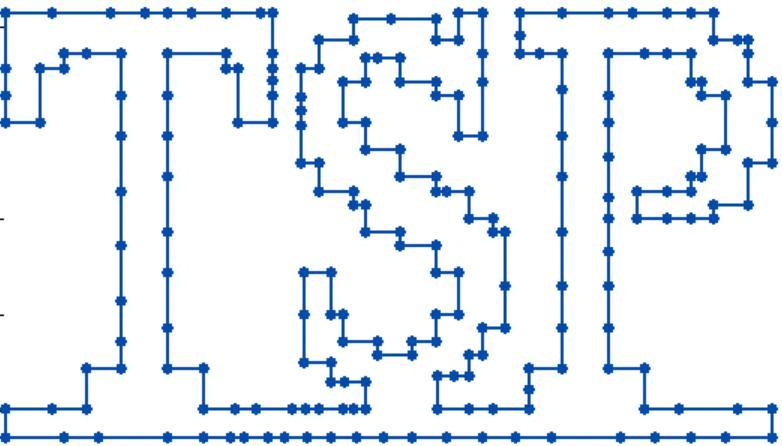
\includegraphics[width=.5\columnwidth]{img/tsp225_plot}
	\caption{The \textit{tsp225.tsp} instance from \textit{tsplib} resolved with \textit{subtour} method described in cap \ref{sec:subtour} plotted by Gnuplot.}
	\label{fig:tsp225}
\end{figure}

The Traveling Salesman Problem is a well-known NP-hard problem. In short, given a set of cities it's required to find the shortest tour that visit exactly one time each city and return to the first one.
In this report two version of the TSP will be analyzed in details:
\begin{itemize}
	\item symmetric TSP (STSP): with bidirectional edges;
 	\item asymmetric TSP (ATSP): with oriented arches.
\end{itemize}


\section{Symmetric TSP}
Given a complete graph $ G = (V, E) $, a distance function $ d $ where:
\begin{itemize}
	\item $ V := \{1, 2, .., n\}$ is a set of nodes;
	\item $ E $ is the set of edges between each node pairs $ i,j \in V, i \ne j $ represented with $ (i,j) $ or for a generic edge $ e $, note that for STSP $ (i,j) = (j,i) $ therefore the number of edges $ |E| = \frac{n(n-1)}{2} $;
	\item $ d: (i,j) = e \to d(i,j) = c_e $ where $ c_e $ is the cost associated to $ e \in E $;
\end{itemize}
and defining the decision variable:
\[
x_e := \begin{cases}
	1 & \text{if $ e $ is in the tour,} \\
	0 & \text{otherwise}
\end{cases}
\] 
the STSP can be represented with linear programming system in \ref{eq:STSP_LP}. 
\begin{equation}
\begin{cases}
		min \sum_{ e\in E } c_ex_e & \text{Cost function} \\
		\sum_{e\in \delta (v) } x_e = 2, \forall v \in V  & \text{Degree constraint} \\
		\sum_{e\in E(S) } x_e \le |S|-1, \forall S \subset V, |S| \ge 3  & \text{Subtour elimination} \\
		x_e \in \{0,1\}, \forall e \in E & \text{Domain constraint}
\end{cases}
\label{eq:STSP_LP}
\end{equation} 
As usual it is required to find the value of $ x_e, \forall e \in E $ that minimize the \textit{cost function} and verify the constraints.
For the \textit{degree constrain}, the degree of each $ v \in V $ ($ |\delta(v)| $) must be equal to 2. A system with only the degree constrain (and the domain constraint) would probably have a set of subtour with size three or more, however adding the \textit{subtour elimination} constraints  it's impose to have only one tour. 

The number of possible subset $ S \subset V $ is exponential ($ 2^{n} - \binom{n}{3} -\binom{n}{2} -\binom{n}{1} - 1 = O(2^n)$), therefore even a graph with 100 nodes has huge matrix dimension. Note that $ E(S) := \{ e = (i,j): i,j \in S \subset V \}$ is the set of edges with both vertices in $ S $.\\
Considering the example in figure \ref{fig:symTSP}, the value of the solution is represented in the matrix in figure \ref{tab:symTSP_solution} where $ x_{ij} = x_{ji} $ for each $ i,j \in V, i \ne j $ but only the cell with $ i < j $ have been completed to enhance the number of variables that are used in practice.

\begin{figure}[h]
	\centering
	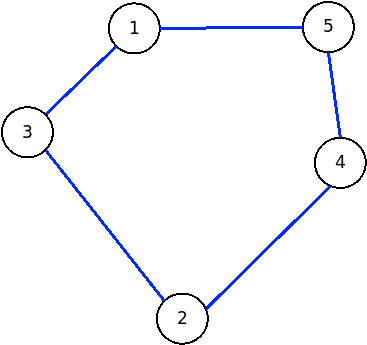
\includegraphics[width=.3\columnwidth]{img/symTSP_example.png}
	\caption{Example of tour. Only the selected edges are visible.}
	\label{fig:symTSP}
\end{figure}

\begin{table}[h!]
	\begin{center}
		\caption{Decision variable matrix. It show the value $ x_{ij} $ of the solution represented in figure \ref{fig:symTSP}. Due to the symmetry of the matrix, only the cell with $ i < j $ have a value, the others can be checked from the first.}
		\label{tab:symTSP_solution}
		\begin{tabular}{cc|c|c|c|c|c|}
			 \multicolumn{2}{c}{} & \multicolumn{5}{c}{j} \\ % <-- Combining two cells with alignment c| and content 12.
			& \multicolumn{1}{c}{} & \multicolumn{1}{c}{1} & \multicolumn{1}{c}{2} & \multicolumn{1}{c}{3} & \multicolumn{1}{c}{4} & \multicolumn{1}{c}{5} \\ \cline{3-7}
			\multirow{5}{*}{i} 	& 1 & \cellcolor{Black} & 0 & 1 & 0 & 1 \\ \cline{3-7}
								& 2 &  & \cellcolor{Black} & 1 & 1 & 0 \\ \cline{3-7}
								& 3 &  &  & \cellcolor{Black} & 0 & 0 \\ \cline{3-7}
								& 4 &  &  &  & \cellcolor{Black} & 1 \\ \cline{3-7}
								& 5 &  &  &  &  & \cellcolor{Black} \\ \cline{3-7}
		\end{tabular}
	\end{center}
\end{table}



\section{Asymmetric TSP}
Given a complete graph $ G = (V,A) $, a distance funciton  $ d $ where:
\begin{itemize}
	\item $ V:= \{1, 2, .., n\} $ is the set of nodes;
	\item $ A := $ the set arches between each nodes $ i,j \in V, i \ne j$ represented as $ (i,j) $, note that in the ATSP $ (i,j) \ne (j,i) $ and the number of arches is $ |A| = n*(n-1) $ which is double of the STSP;
	\item $ d: (i,j) \rightarrow d(i,j) = c_{ij} $ where $ c_{ij} $ is the cost associated to the arch $ (i,j) $.
\end{itemize}
As in the STSP, it is defined the decision variable $ x_{ij} $ which tell if the arch $ (i,j) $ is in the tour:
\[
x_{ij} := \begin{cases}
1 & \text{if $ (i,j) $ is in the tour,} \\
0 & \text{otherwise}
\end{cases}
\]

The ATSP can be defined in different ways, in this report two version will be considered in detail: Miller Tucker Zemlin and Flow Chart (by GG). % TODO: find the name of the author % 

\subsection{Miller Tucker Zemlin}
Miller Tucker Zemlin (MTZ) model impose the "subtour elimination" constraints with the help of another decision variable $ u_k $. For each node $ k = 2,..,n $, $ u_k $ is the position of the node $ k $ in the tour that start from the node $ 1 $. As an example in fig \ref{fig:asymTSP_MTZ} it is shown that $ u_1 = 0 $ and than $ u_k $ increase until $ n-1 $ along the tour.

\begin{figure}[h]
	\centering
	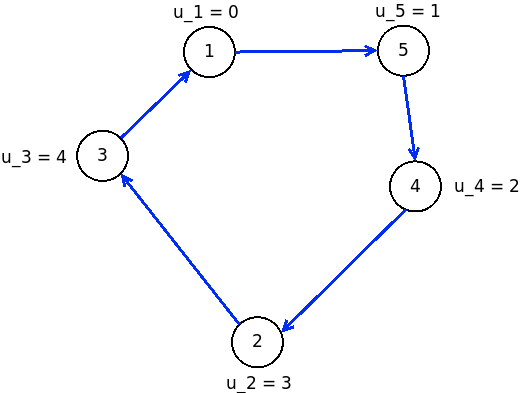
\includegraphics[width=.45\columnwidth]{img/asymTSP_MTZ_example.png}
	\caption{Example of tour. Only the selected arches are visible.}
	\label{fig:asymTSP_MTZ}
\end{figure}

The proposed model is shown in the system \ref{eq:ATSP_MTZ}. The cost function and the degree constraints are adapted to the asymmetric problem, moreover MTZ constraint is derived from $ u_j \ge u_i+1-M(1-x_{ij}), \forall i,j \in V \backslash \{1\}, M >> 0 $. Considering an arch $ (i,j) \in A \backslash \{1\} $ if it is in the tour then $ u_j \ge u_i + 1 $ because $ M(1-x_{ij}) = 0 $, else $ u_j \ge u_i + 1 - M < 0 \implies u_j \ge 0 $. For example for the arch $ (4,2) $ in fig \ref{fig:asymTSP_MTZ}, $ 3 \ge 2 + 1 - M(1-1) \iff 3 \ge 3 $. \\

\begin{equation}
\begin{cases}
min \sum_{i\in V}\sum_{j\in V} c_{ij}x_{ij} & \text{Cost function} \\
\sum_{i\in V} x_{ih} = 1, \forall h \in V  & \text{$ x $ Outer arches degree} \\
\sum_{i\in V} x_{hi} = 1, \forall h \in V  & \text{$ x $ Inner arches degree} \\
u_i -u_j +M x_{ij} \le M - 1, \forall i,j \in V \backslash \{1\} & \text{MTZ constraints ($ O(n^2) $)} \\
0 \le x_{ij} \le 1, Integer, \forall i,j \in N  & \text{$ x $ Domain} \\
0 \le x_{ii} \le 0, Integer, \forall i \in N  & \text{} \\
0 \le u_{i} \le n-2, Integer, \forall i \in N \backslash \{1\} & \text{$ u $ Domain} 
\end{cases}
\label{eq:ATSP_MTZ}
\end{equation}


Note that the number of MTZ constraints is $ O(n^2) $, one for each arch, therefore much less respect STSP model.\\
The number of decision variables instead is more than the double $ n(n-1) + n = n^2 $. Computational consideration will be done in the next chapter.

\begin{table}[h!]
	\begin{center}$  $
		\caption{Decision variable matrix. It show the value $ x_{ij} $ and $ u_k $ of the solution represented in figure \ref{fig:asymTSP_MTZ}. }
		\label{tab:asymTSP_MTZ_solution}
		\begin{tabular}{cc|c|c|c|c|c|}
			 $ x_{ij} $ & \multicolumn{1}{c}{} & \multicolumn{5}{c}{j} \\ % <-- Combining two cells with alignment c| and content 12.
			& \multicolumn{1}{c}{} & \multicolumn{1}{c}{1} & \multicolumn{1}{c}{2} & \multicolumn{1}{c}{3} & \multicolumn{1}{c}{4} & \multicolumn{1}{c}{5} \\ \cline{3-7}
			\multirow{5}{*}{i} 	& 1 & \cellcolor{Black} & 0 & 0 & 0 & 1 \\ \cline{3-7}
			& 2 & 0 & \cellcolor{Black} & 1 & 0 & 0 \\ \cline{3-7}
			& 3 & 1 & 0 & \cellcolor{Black} & 0 & 0 \\ \cline{3-7}
			& 4 & 0 & 1 & 0 & \cellcolor{Black} & 0 \\ \cline{3-7}
			& 5 & 0 & 0 & 0 & 1 & \cellcolor{Black} \\ \cline{3-7}
			\multicolumn{7}{c}{} \\ 
			
			\multicolumn{2}{c}{} & \multicolumn{5}{c}{$ k $} \\  
			& \multicolumn{1}{c}{} & \multicolumn{1}{c}{1} & \multicolumn{1}{c}{2} & \multicolumn{1}{c}{3} & \multicolumn{1}{c}{4} & \multicolumn{1}{c}{5} \\ \cline{3-7}
 			$ u_k $ &  & 0 & 3 & 4 & 2 & 1 \\ \cline{3-7}
		\end{tabular}
	\end{center}
\end{table}

\subsection{Flow Chart}
The Flow Chart model impose the "subtour elimination" constraints with a decision variable $ y_{ij} $ which is associated to each arch $ (i,j) \in V $ and represent a flow that decrease from $ n-1 $ to $ 0 $ each node of the tour and is $ 0 $ if it is not in the tour. As shown in fig \ref{fig:asymTSP_FC} starting from the node $ 1 $ the flow $ y_{15} = 4 $ than decrease each step by $ 1 $ unit until the last arch of the tour where $ y_{31} = 0 $. Note that the last arch $ y_{31} $ has the same value of the unselected one, this is because the last arch of the tour is implicit. \\
The proposed LP model is in eq \ref{eq:ATSP_FC}. The outer flow of $ 1 $ is the first constraint, than to make the flow decrease it is imposed the "flow equilibrium" where each inner flow must be equal to the outer flow $ +1 $ and, in the end, "the cuttling constraints" imposed that only the arches in the tour can have $ y > 0 $ otherwise must be equal to $ 0 $. The last set of constraint force the flow to move along the tour and decrease each step. \\

\begin{equation}
\begin{cases}
min \sum_{i\in V}\sum_{j\in V} c_{ij}x_{ij}  & \text{Cost function} \\
\sum_{i\in V} x_{ih} = 1, \forall h \in V  & \text{$ x $ Outer arches} \\
\sum_{i\in V} x_{hi} = 1, \forall h \in V  & \text{$ x $ Inner arches} \\
\sum_{j\in V} y_{1j} = n-1  & \text{$ 1 $ Outer flow} \\
\sum_{j\in V} y_{hj} = \sum_{i \in V}y_{ih} - 1, \forall h \in V \backslash \{1\}  & \text{Flow equilibrium} \\
y_{ij} - x_{ij}(n-1) \le 0, \forall i \in V, \forall j \in V \backslash \{1\}  & \text{Cuttling constraints} \\ % TODO: is correct the name of the constraints?%
0 \le x_{ij} \le 1, Integer, \forall i,j \in N  & \text{$ x $ Domain} \\
0 \le x_{ii} \le 0, Integer, \forall i \in N & \text{} \\
0 \le y_{i1} \le 0, \forall i \in V  & \text{$ y $ Domain} \\
0 \le y_{ii} \le 0, \forall i \in V  & \text{} \\
0 \le y_{ij} \le n-1, Integer, \forall i,j \in V  & \text{} 
\end{cases}
\label{eq:ATSP_FC}
\end{equation}


The number of FC constraint equals to $ O(1) + O(n-1) + O(n^2) = O(n^2) $. The tables of variable are shown in tab \ref{tab:asymTSP_FC_solution} with the associated solution example in fig \ref{fig:asymTSP_FC}. It's easy to see that the number of variable is $ 2n(n-1) = O(n^2) $\\


\begin{figure}[h]
	\centering
	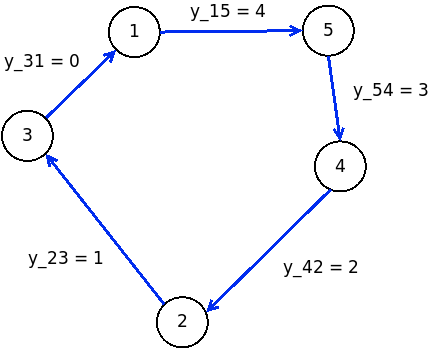
\includegraphics[width=.45\columnwidth]{img/asymTSP_FC_example.png}
	\caption{Example of tour. Only the selected arches are visible.}
	\label{fig:asymTSP_FC}
\end{figure}

\begin{table}[h!]
	\begin{center}
		\caption{Decision variable matrix. It show the value $ x_{ij}, y_{ij} $ of the solution represented in figure \ref{fig:asymTSP_FC}.}
		\label{tab:asymTSP_FC_solution}
		\begin{tabular}{cc|c|c|c|c|c|}
			
$ x_{ij} $ & \multicolumn{1}{c}{} & \multicolumn{5}{c}{j} \\ % <-- Combining two cells with alignment c| and content 12.
& \multicolumn{1}{c}{} & \multicolumn{1}{c}{1} & \multicolumn{1}{c}{2} & \multicolumn{1}{c}{3} & \multicolumn{1}{c}{4} & \multicolumn{1}{c}{5} \\ \cline{3-7}
\multirow{5}{*}{i} 	& 1 & \cellcolor{Black} & 0 & 0 & 0 & 1 \\ \cline{3-7}
& 2 & 0 & \cellcolor{Black} & 1 & 0 & 0 \\ \cline{3-7}
& 3 & 1 & 0 & \cellcolor{Black} & 0 & 0 \\ \cline{3-7}
& 4 & 0 & 1 & 0 & \cellcolor{Black} & 0 \\ \cline{3-7}
& 5 & 0 & 0 & 0 & 1 & \cellcolor{Black} \\ \cline{3-7}
\multicolumn{7}{c}{} \\ 

$ y_{ij} $ & \multicolumn{1}{c}{} & \multicolumn{5}{c}{j} \\ % <-- Combining two cells with alignment c| and content 12.
& \multicolumn{1}{c}{} & \multicolumn{1}{c}{1} & \multicolumn{1}{c}{2} & \multicolumn{1}{c}{3} & \multicolumn{1}{c}{4} & \multicolumn{1}{c}{5} \\ \cline{3-7}
\multirow{5}{*}{i} 	& 1 & \cellcolor{Black} & 0 & 0 & 0 & 4 \\ \cline{3-7}
					& 2 & 0 & \cellcolor{Black} & 0 & 0 & 0 \\ \cline{3-7}
					& 3 & 1 & 0 & \cellcolor{Black} & 0 & 0 \\ \cline{3-7}
					& 4 & 0 & 2 & 0 & \cellcolor{Black} & 0 \\ \cline{3-7}
					& 5 & 0 & 0 & 0 & 3 & \cellcolor{Black} \\ \cline{3-7}
			
		\end{tabular}
	\end{center}
\end{table}